\documentclass[12pt, titlepage]{article}

\usepackage{booktabs}
\usepackage{tabularx}
\usepackage{hyperref}
\hypersetup{
    colorlinks,
    citecolor=black,
    filecolor=black,
    linkcolor=red,
    urlcolor=blue
}
\usepackage[round]{natbib}
\usepackage{geometry}

\usepackage{adjustbox}
\usepackage[dvipsnames]{xcolor}
\usepackage{float}
\usepackage{changepage}
\usepackage{pdflscape}

%% Comments

\usepackage{color}

\newif\ifcomments\commentstrue %displays comments
%\newif\ifcomments\commentsfalse %so that comments do not display

\ifcomments
\newcommand{\authornote}[3]{\textcolor{#1}{[#3 ---#2]}}
\newcommand{\todo}[1]{\textcolor{red}{[TODO: #1]}}
\else
\newcommand{\authornote}[3]{}
\newcommand{\todo}[1]{}
\fi

\newcommand{\wss}[1]{\authornote{blue}{SS}{#1}} 
\newcommand{\plt}[1]{\authornote{magenta}{TPLT}{#1}} %For explanation of the template
\newcommand{\an}[1]{\authornote{cyan}{Author}{#1}}

%% Common Parts

\newcommand{\progname}{Software Engineering} % PUT YOUR PROGRAM NAME HERE
\newcommand{\authname}{Team \#13, ARC
    \\ Avanish, Ahluwalia
    \\ Russell, Davidson
    \\ Rafey, Malik
    \\ Abdul, Zulfiqar} % AUTHOR NAMES                  

\usepackage{hyperref}
    \hypersetup{colorlinks=true, linkcolor=blue, citecolor=blue, filecolor=blue,
                urlcolor=blue, unicode=false}
    \urlstyle{same}
                                


\begin{document}

\title{Verification and Validation Report: \progname}
\author{\authname}
\date{\today}

\maketitle

\pagenumbering{roman}

\section{Revision History}

\begin{tabularx}{\textwidth}{p{3cm}p{2cm}X}
  \toprule {\bf Date} & {\bf Version} & {\bf Notes} \\
  \midrule
  Date 1              & 1.0           & Notes       \\
  Date 2              & 1.1           & Notes       \\
  \bottomrule
\end{tabularx}

~\newpage

\section{Symbols, Abbreviations and Acronyms}

\renewcommand{\arraystretch}{1.2}
\begin{tabular}{l l}
  \toprule
  \textbf{symbol} & \textbf{description} \\
  \midrule
  T               & Test                 \\
  \bottomrule
\end{tabular}\\

\wss{symbols, abbreviations or acronyms -- you can reference the SRS tables if needed}

\newpage

\tableofcontents

\listoftables %if appropriate

\listoffigures %if appropriate

\newpage

\pagenumbering{arabic}

This document ...

\section{Functional Requirements Evaluation}

\subsection{Database Testing}
The following section presents the results of the our database testing


\begin{table}[H]
  \caption{\bf Functional Requirements Evaluation Results for Database Testing}
  \resizebox{6in}{!}{\begin{tabular}{|l|p{0.15\linewidth}|p{0.3\linewidth}|p{0.3\linewidth}|p{0.3\linewidth}|p{0.1\linewidth}|}
      \hline
      \multicolumn{1}{|l|}{\bfseries Id} & \multicolumn{1}{|l|}{\bfseries Type} & \multicolumn{1}{l|}{\bfseries Inputs}                                      & \multicolumn{1}{l|}{\bfseries Expected Result}                              & \multicolumn{1}{l|}{\bfseries Actual Result} & \multicolumn{1}{l|}{\bfseries Result} \\
      \hline
      Test-DB1                           & Automated                            & Periodic backup run is completed.                                          & Automated monitor verifies that the database backup is present and correct. & Same as expected                             & \textcolor{Green}{Pass}               \\
      \hline
      Test-DB2                           & Automated                            & Command to check encryption status is inputted into DBMS for all databases & DBMS response shows that all databases are encrypted                        & Same as expected                             & \textcolor{Green}{Pass}               \\
      \hline
    \end{tabular}}
  \label{table:GR1}
\end{table}

\subsection{Custom AR Object Generation}
The following section presents the results of our custom AR object generation testing.

\begin{table}[H]
  \caption{\bf Functional Requirements Evaluation Results for Custom AR Object Generation}
  \resizebox{6in}{!}{\begin{tabular}{|l|p{0.15\linewidth}|p{0.3\linewidth}|p{0.3\linewidth}|p{0.3\linewidth}|p{0.1\linewidth}|}
      \hline
      \multicolumn{1}{|l|}{\bfseries Id} & \multicolumn{1}{|l|}{\bfseries Control} & \multicolumn{1}{l|}{\bfseries Inputs}                         & \multicolumn{1}{l|}{\bfseries Expected Result}                                                                     & \multicolumn{1}{l|}{\bfseries Actual Result} & \multicolumn{1}{l|}{\bfseries Result} \\
      \hline
      Test-POG1                          & Automatic                               & Enter prompts of various lengths, with and without profanity. & Prompt is restricted to 200 characters, real-time character count is displayed, profanity is flagged and rejected. & Same as expected                             & \textcolor{Green}{Pass}               \\
      \hline
      Test-POG5                          & Manual                                  & Rotate the AR object to inspect all sides.                    & The AR object rotates smoothly, allowing inspection from all angles.                                               & Same as expected                             & \textcolor{Green}{Pass}               \\
      \hline
    \end{tabular}}
  \label{table:GR2}
\end{table}

\subsection{Uploading Objects to Inventory, Post Object Scan}
The following section presents the results of our testing for uploading objects to inventory after scanning.

\begin{table}[H]
  \caption{\bf Functional Requirements Evaluation Results for Uploading Objects to Inventory}
  \resizebox{6in}{!}{\begin{tabular}{|l|p{0.15\linewidth}|p{0.3\linewidth}|p{0.3\linewidth}|p{0.3\linewidth}|p{0.1\linewidth}|}
      \hline
      \multicolumn{1}{|l|}{\bfseries Id} & \multicolumn{1}{|l|}{\bfseries Control} & \multicolumn{1}{l|}{\bfseries Inputs}                                      & \multicolumn{1}{l|}{\bfseries Expected Result}                                & \multicolumn{1}{l|}{\bfseries Actual Result} & \multicolumn{1}{l|}{\bfseries Result} \\
      \hline
      Test-OUI1                          & Manual                                  & Display the scanned object and allow for user interaction in editing mode. & Render of scanned object is displayed, user can edit and finalize the object. & Same as expected                             & \textcolor{Green}{Pass}               \\
      \hline
      Test-OUI2                          & Manual                                  & Provide a name for the object and save it with metadata.                   & Object name is stored (ASCII only), and all metadata is correctly saved.      & Same as expected                             & \textcolor{Green}{Pass}               \\
      \hline
      Test-OUI3                          & Manual                                  & Select specific portions of the object and apply color changes.            & Color changes are applied accurately and reflected in the final render.       & Same as expected                             & \textcolor{Green}{Pass}               \\
      \hline
    \end{tabular}}
  \label{table:GR3}
\end{table}

\restoregeometry

\section{Nonfunctional Requirements Evaluation}
\subsection{Usability Testing}
The following section presents the results of our usability testing.

\begin{table}[H]
  \caption{\bf Usability Testing Evaluation Results}
  \resizebox{6in}{!}{\begin{tabular}{|l|p{0.15\linewidth}|p{0.3\linewidth}|p{0.3\linewidth}|p{0.3\linewidth}|p{0.1\linewidth}|}
      \hline
      \multicolumn{1}{|l|}{\bfseries Id} & \multicolumn{1}{|l|}{\bfseries Type} & \multicolumn{1}{l|}{\bfseries Inputs}                                         & \multicolumn{1}{l|}{\bfseries Expected Result}                                   & \multicolumn{1}{l|}{\bfseries Actual Result} & \multicolumn{1}{l|}{\bfseries Result} \\
      \hline
      Test-QS-U1                         & Manual                               & Language setting is changed to English, Mandarin, Hindi, Spanish, and French. & Text updates correctly in all tested languages with understandable translations. & Same as expected                             & \textcolor{Green}{Pass}               \\
      \hline
      Test-QS-U2                         & Manual                               & New users perform core app workflows without guidance.                        & 80\% of testers complete tasks and rate the app as intuitive and satisfying.     & Same as expected                             & \textcolor{Green}{Pass}               \\
      \hline
    \end{tabular}}
  \label{table:GR-Usability}
\end{table}

\subsection{Security Testing}
The following section presents the results of our security testing.

\begin{table}[H]
  \caption{\bf Security Testing Evaluation Results}
  \resizebox{6in}{!}{\begin{tabular}{|l|p{0.15\linewidth}|p{0.3\linewidth}|p{0.3\linewidth}|p{0.3\linewidth}|p{0.1\linewidth}|}
      \hline
      \multicolumn{1}{|l|}{\bfseries Id} & \multicolumn{1}{|l|}{\bfseries Type} & \multicolumn{1}{l|}{\bfseries Inputs}                                        & \multicolumn{1}{l|}{\bfseries Expected Result}     & \multicolumn{1}{l|}{\bfseries Actual Result} & \multicolumn{1}{l|}{\bfseries Result} \\
      \hline
      Test-QS-SC3                        & Manual                               & Code sections displaying private data are checked for identity verification. & All sections contain identity verification checks. & Same as expected                             & \textcolor{Green}{Pass}               \\
      \hline
    \end{tabular}}
  \label{table:GR-Security}
\end{table}

\subsection{Availability Testing}
The following section presents the results of our availability testing.

\begin{table}[H]
  \caption{\bf Availability Testing Evaluation Results}
  \resizebox{6in}{!}{\begin{tabular}{|l|p{0.15\linewidth}|p{0.3\linewidth}|p{0.3\linewidth}|p{0.3\linewidth}|p{0.1\linewidth}|}
      \hline
      \multicolumn{1}{|l|}{\bfseries Id} & \multicolumn{1}{|l|}{\bfseries Type} & \multicolumn{1}{l|}{\bfseries Inputs} & \multicolumn{1}{l|}{\bfseries Expected Result} & \multicolumn{1}{l|}{\bfseries Actual Result} & \multicolumn{1}{l|}{\bfseries Result} \\
      \hline
      Test-QS-A1                         & Automated                            & Monitor server uptime over one week.  & Server uptime recorded at 99\% or higher.      & Same as expected                             & \textcolor{Green}{Pass}               \\
      \hline
    \end{tabular}}
  \label{table:GR-Availability}
\end{table}


\subsection{Performance}

\subsection{etc.}

\section{Comparison to Existing Implementation}

This section will not be appropriate for every project.

\section{Unit Testing}

\section{Changes Due to Testing}

\wss{This section should highlight how feedback from the users and from
  the supervisor (when one exists) shaped the final product.  In particular
  the feedback from the Rev 0 demo to the supervisor (or to potential users)
  should be highlighted.}

\section{Automated Testing}

\section{Trace to Requirements}

\section{Trace to Modules}

\section{Code Coverage Metrics}

\bibliographystyle{plainnat}
\bibliography{../../refs/References}

\newpage{}
\section*{Appendix --- Usability Survey Results}

\textbf{Link to view survey: \href{https://docs.google.com/forms/d/e/1FAIpQLSdlrjJkx5uAdkjsMwDsV0cWCIpfhzvdnSnNukdR0-1SlWtrtA/viewform?usp=dialog}{here}}

Table \ref{table:US1} below showing the results of the Usability survey

\newgeometry{left=2cm,bottom=0.1cm}
\begin{table}[htbp]
  \caption{\bf Results of Usability Survey}
  \resizebox{6.5in}{!}{\begin{tabular}{|p{0.4\linewidth}|p{0.3\linewidth}|p{0.7\linewidth}|}
      \hline
      {\bfseries Statement}                         & {\bfseries Average Rating of Statement Accuracy / 5} & {\bfseries Analysis}                                                                                                                                                               \\
      \hline
      Navigation between interfaces is intuitive    & 3.833                                                & Most users found the navigation to be intuitive, although navigation seems to be the lowest rated aspect of the functional user experience                                         \\
      \hline
      Placing objects is easy                       & 3.917                                                & No ratings below a three and an average rating of "Agree" says that this was well recieved                                                                                         \\
      \hline
      Generating objects is easy                    & 3.917                                                & Again, no ratings below a three and an average rating of "Agree" indicates that the design works for most users                                                                    \\
      \hline
      It is easy to start a tour                    & 4.167                                                & A good indication that the touring experience was designed well                                                                                                                    \\
      \hline
      Changing settings is easy                     & 4.417                                                & Somewhat expected, users generally did not have issues finding and changing settings as it was a straightforward feature                                                           \\
      \hline
      The app is generally satisfying to use        & 3.667                                                & This was the lowest rating of all our positive statements. We recieved relevant feedback on the non-uniform look and feel of the app making the app feel like a rushed development \\
      \hline
      Using the app distracts from the surroundings & 3.167                                                & More found the app distracting than not, but the results are somewhat inconclusive given the variance                                                                              \\
      \hline
    \end{tabular}}
  \label{table:US1}
\end{table}

\begin{figure}[htbp]
  \caption{"Navigation between interfaces is intuitive" statement ratings}
  \centerline{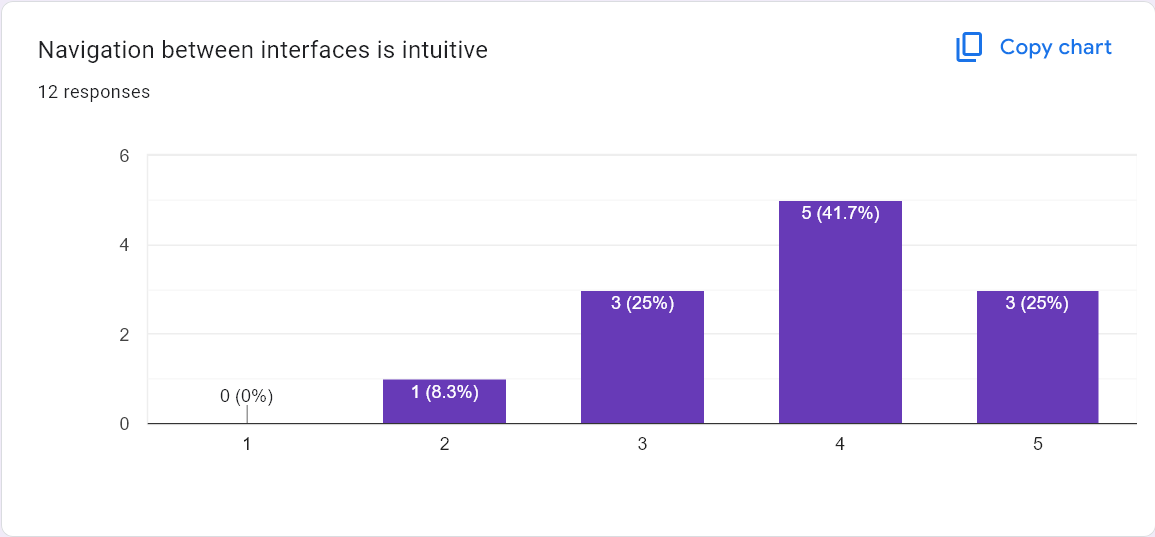
\includegraphics[scale=0.35]{./Images/Q1.png}}
  \label{fig:StraightForward}
\end{figure}

\begin{figure}[htbp]
  \caption{"Placing objects is easy" statement ratings}
  \centerline{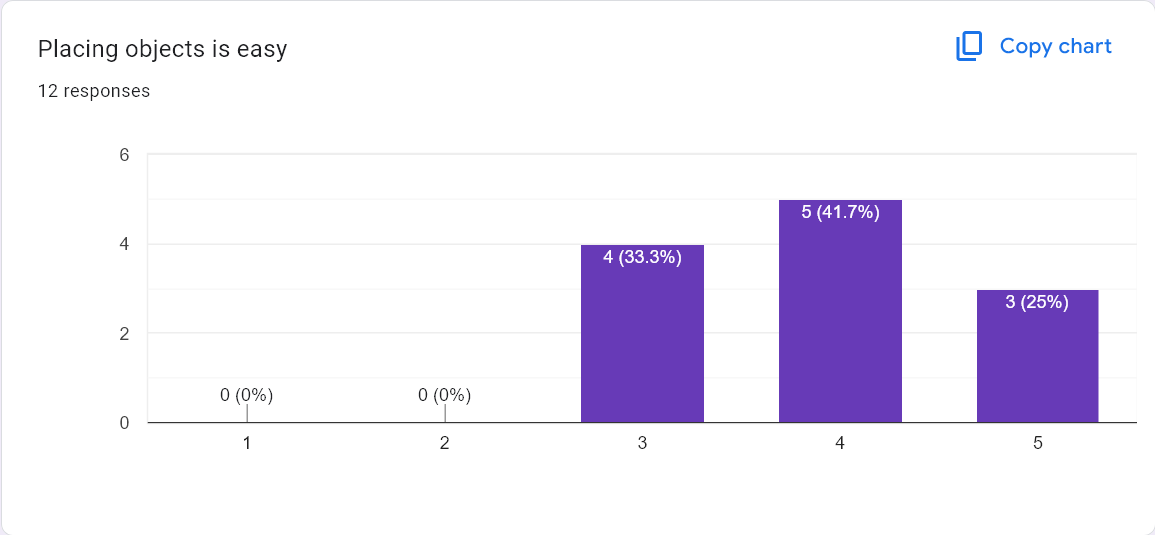
\includegraphics[scale=0.35]{./Images/Q2.png}}
  \label{fig:Navigation}
\end{figure}

\begin{figure}[htbp]
  \caption{"Generating objects is easy" statement ratings}
  \centerline{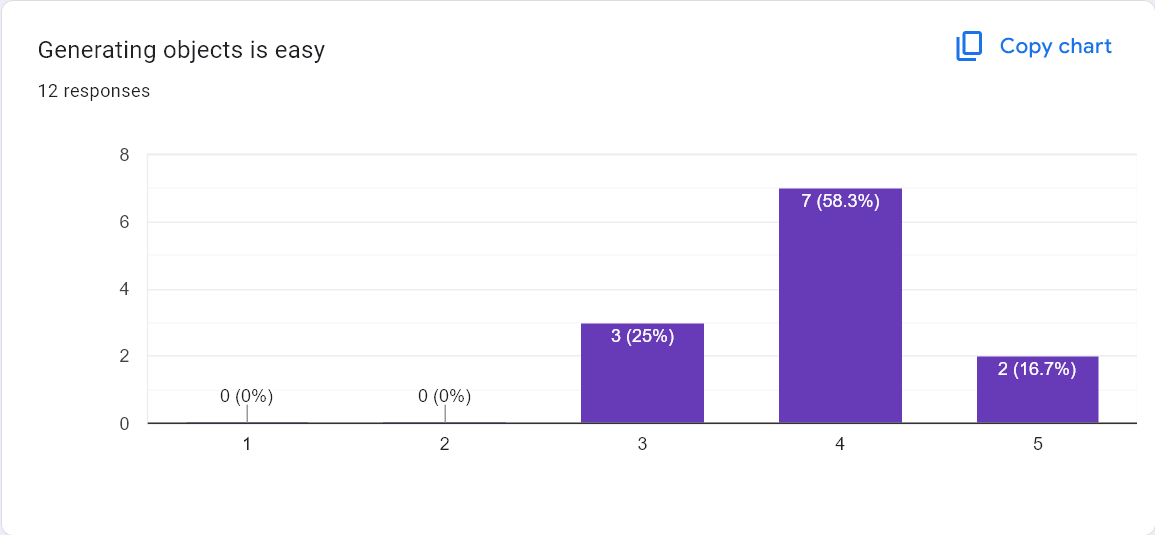
\includegraphics[scale=0.35]{./Images/Q3.png}}
  \label{fig:Detached}
\end{figure}

\begin{figure}[htbp]
  \caption{"It is easy to start a tour" statement ratings}
  \centerline{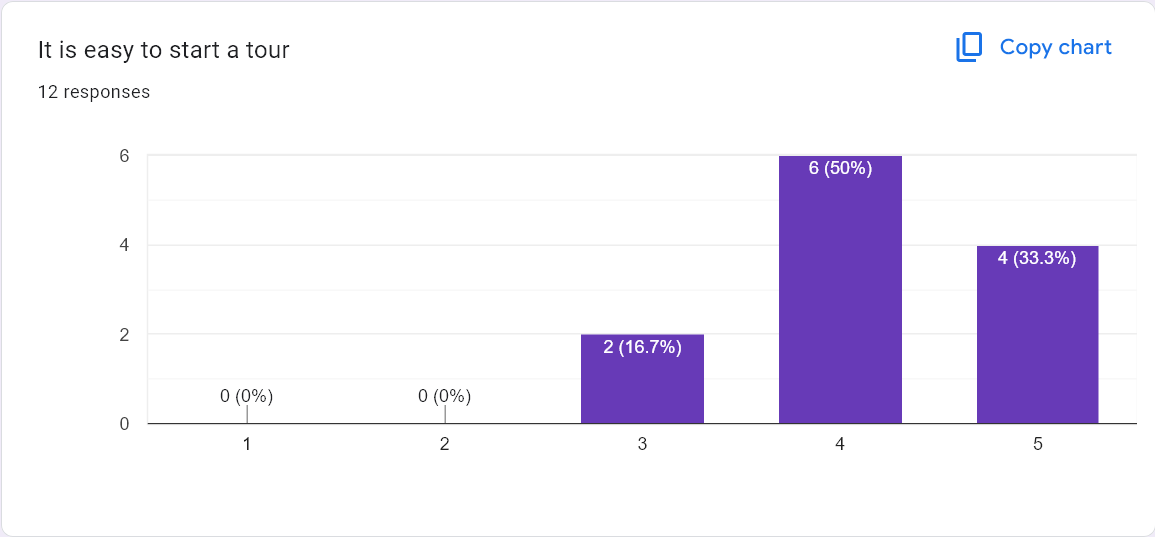
\includegraphics[scale=0.35]{./Images/Q4.png}}
  \label{fig:RealWorld}
\end{figure}

\begin{figure}[htbp]
  \caption{"Changing settings is easy" statement ratings}
  \centerline{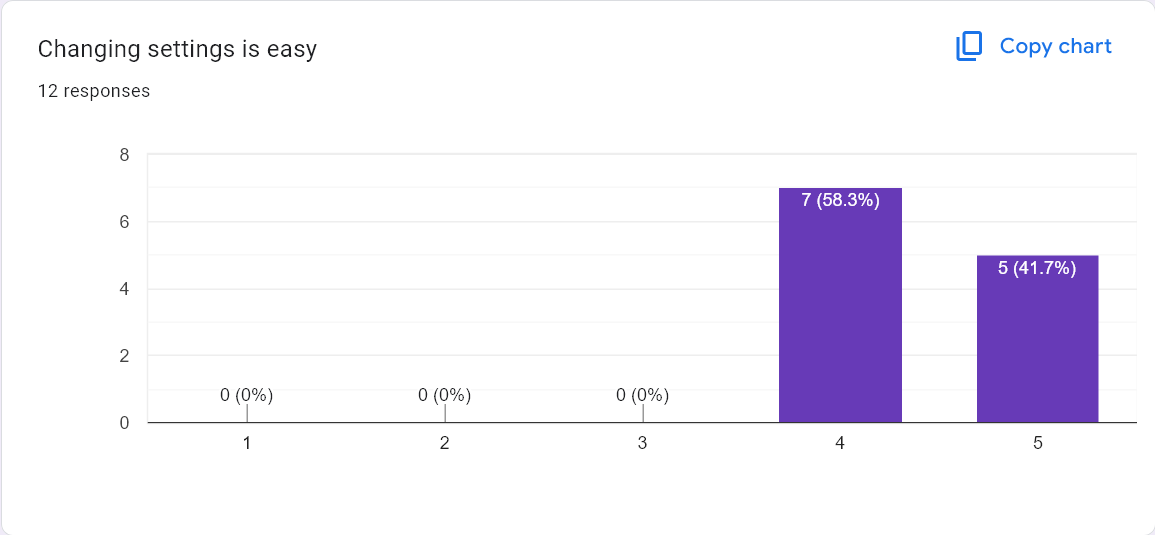
\includegraphics[scale=0.35]{./Images/Q5.png}}
  \label{fig:Fun}
\end{figure}

\begin{figure}[htbp]
  \caption{"The app is generally satisfying to use" statement ratings}
  \centerline{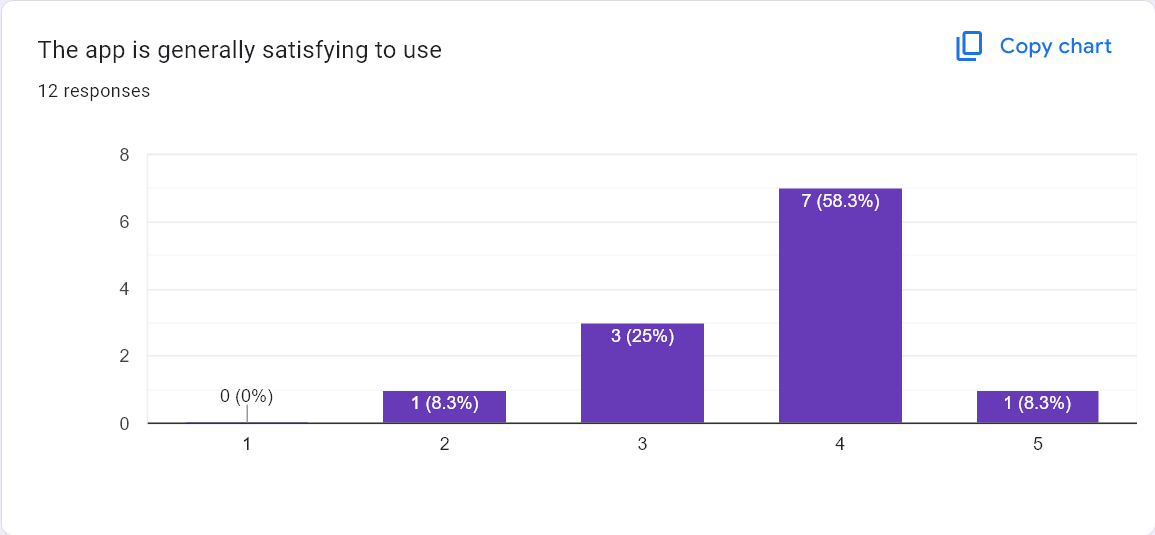
\includegraphics[scale=0.35]{./Images/Q6.png}}
  \label{fig:Social}
\end{figure}

\begin{figure}[htbp]
  \caption{"Using the app distracts from the surroundings" statement ratings}
  \centerline{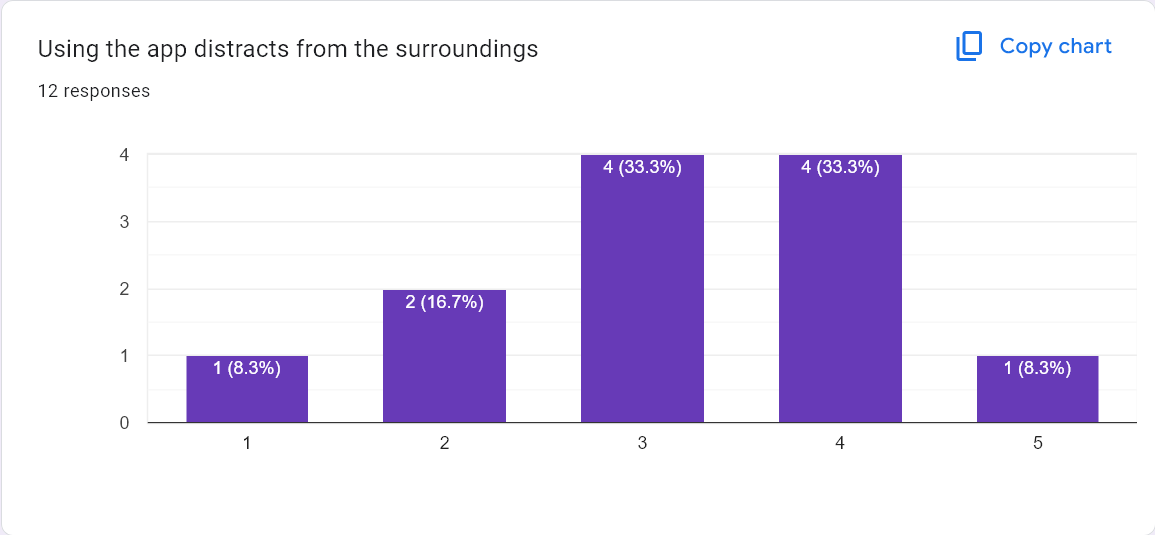
\includegraphics[scale=0.35]{./Images/Q7.png}}
  \label{fig:Enjoy}
\end{figure}

\newpage{}

\section*{Appendix --- Reflection}

The information in this section will be used to evaluate the team members on the
graduate attribute of Reflection.

The purpose of reflection questions is to give you a chance to assess your own
learning and that of your group as a whole, and to find ways to improve in the
future. Reflection is an important part of the learning process.  Reflection is
also an essential component of a successful software development process.  

Reflections are most interesting and useful when they're honest, even if the
stories they tell are imperfect. You will be marked based on your depth of
thought and analysis, and not based on the content of the reflections
themselves. Thus, for full marks we encourage you to answer openly and honestly
and to avoid simply writing ``what you think the evaluator wants to hear.''

Please answer the following questions.  Some questions can be answered on the
team level, but where appropriate, each team member should write their own
response:


\begin{enumerate}
  \item What went well while writing this deliverable?
  \item What pain points did you experience during this deliverable, and how
        did you resolve them?
  \item Which parts of this document stemmed from speaking to your client(s) or
        a proxy (e.g. your peers)? Which ones were not, and why?
  \item In what ways was the Verification and Validation (VnV) Plan different
        from the activities that were actually conducted for VnV?  If there were
        differences, what changes required the modification in the plan?  Why did
        these changes occur?  Would you be able to anticipate these changes in future
        projects?  If there weren't any differences, how was your team able to clearly
        predict a feasible amount of effort and the right tasks needed to build the
        evidence that demonstrates the required quality?  (It is expected that most
        teams will have had to deviate from their original VnV Plan.)
\end{enumerate}

\end{document}